\label{expr_e000}
In this chapter, we'll discuss about how to evaluate
C language expression and how to generate 3 address code
discussed in chapter \ref{_3ac_e001}.

In the section \ref{symtab_e003}, we didn't mention about {\tt{var}} 
which is data structure of the compiler medium variable, or other
classes derved from {\tt{var}}. Now here, we'll illustrate
the based or derived relation in figure \ref{expr_e013}.
In later section, we'll refer to the usage of these classes.

\begin{figure}[htbp]
\begin{center}
%%\begin{htmlonly}
%%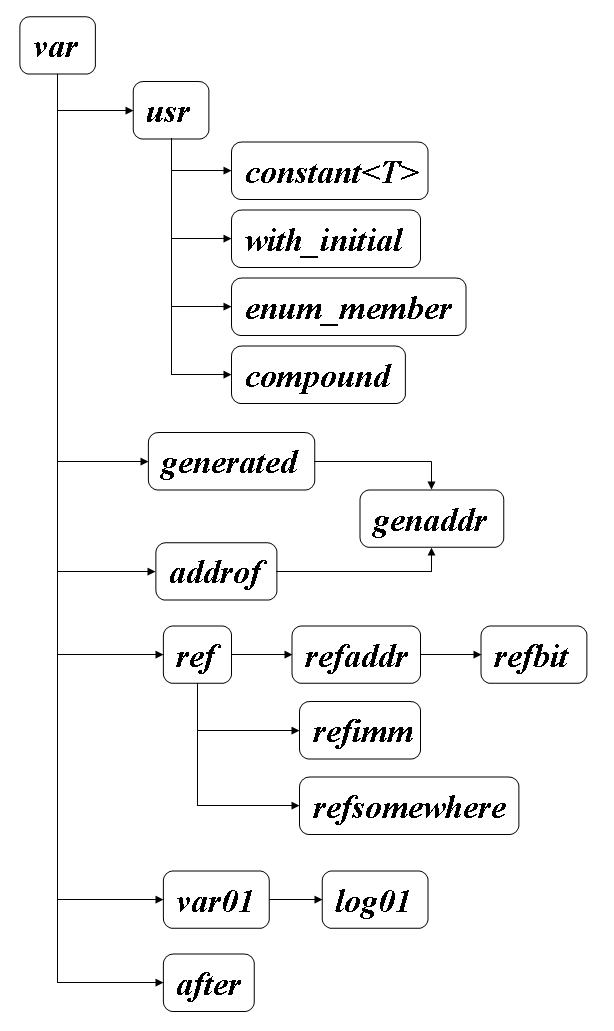
\includegraphics[width=1.0\linewidth,height=1.626\linewidth]{var.png}
%%\end{htmlonly} 
%%\begin{latexonly}
%%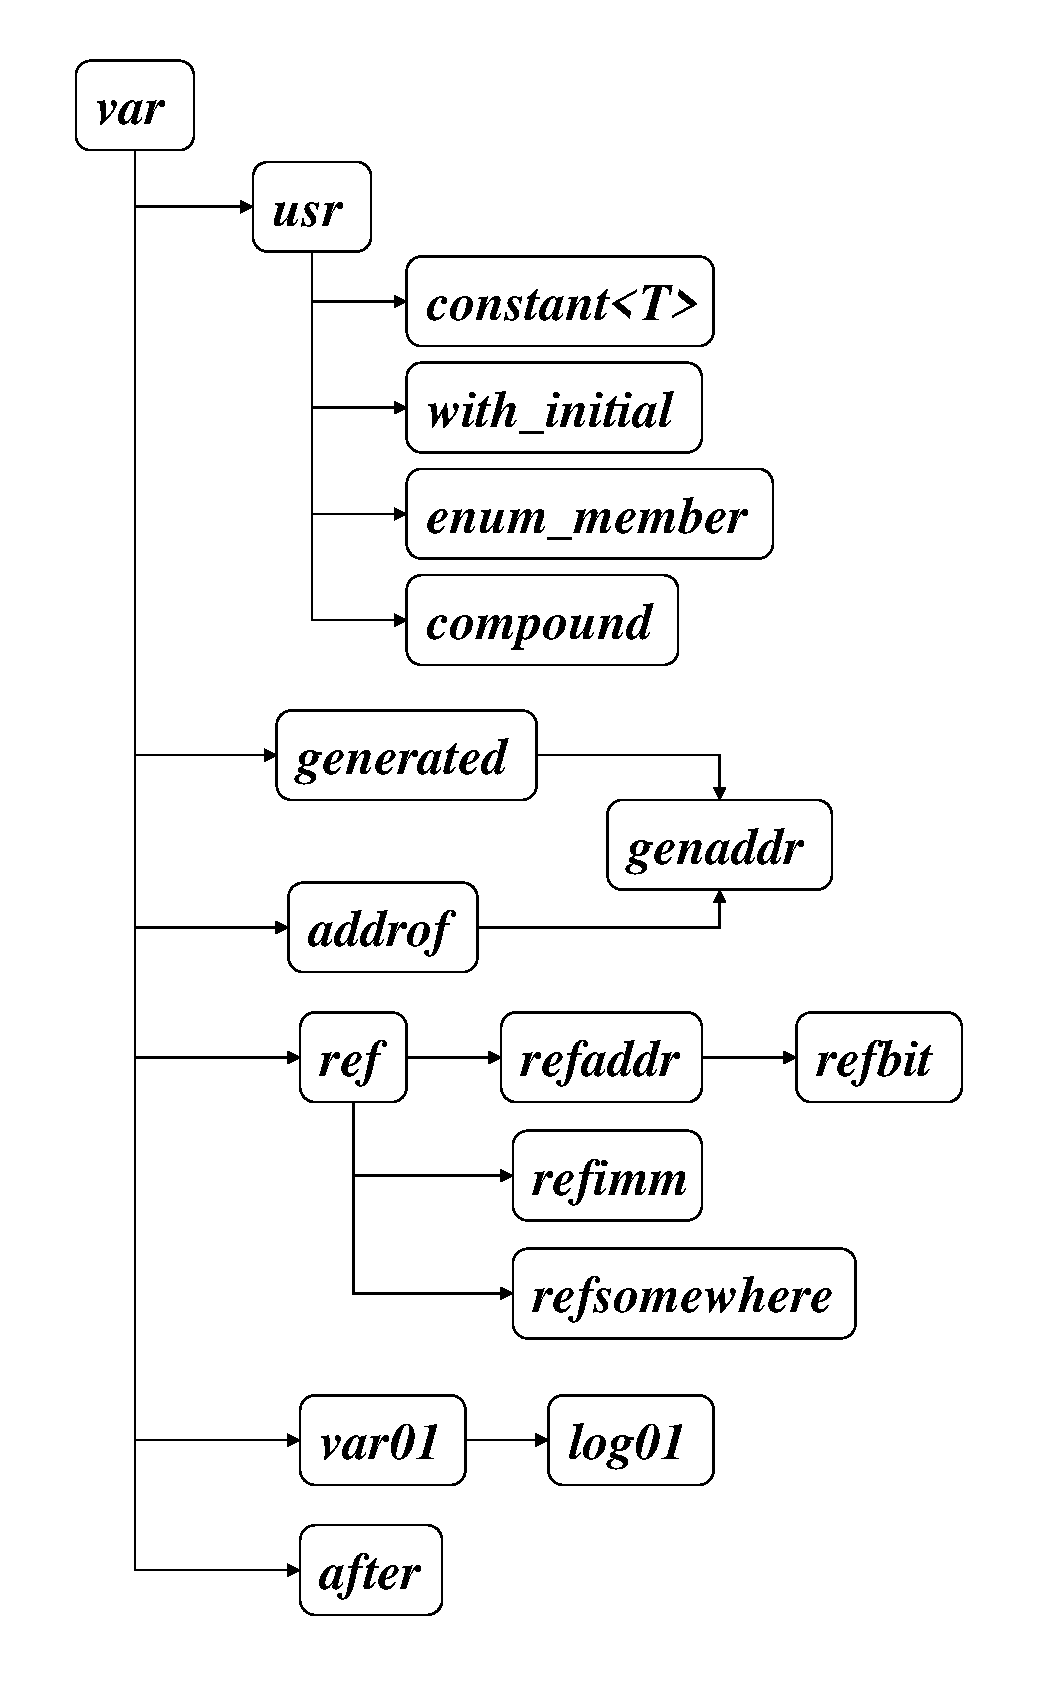
\includegraphics[width=1.0\linewidth,height=1.626\linewidth]{var.eps}
%%\includegraphics[width=1.8\linewidth,height=2.35\linewidth]{var2.eps}
%%\includegraphics[width=1.5\linewidth,height=1.5\linewidth]{var3.eps}
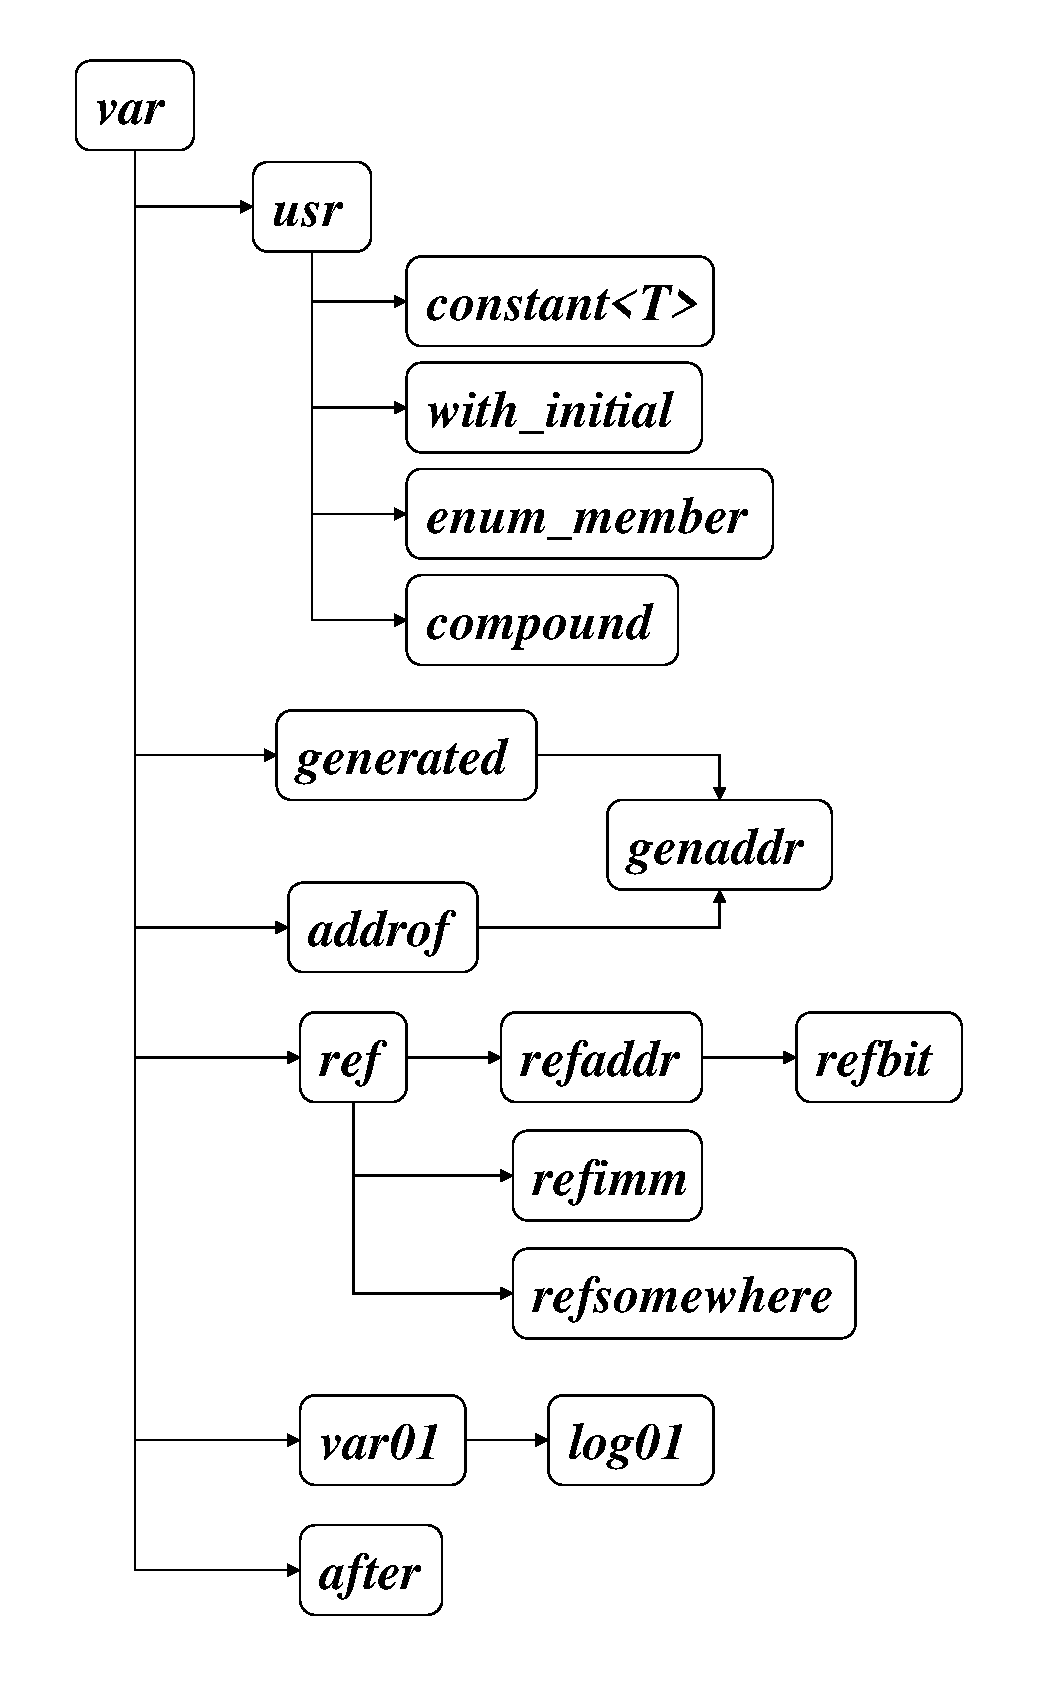
\includegraphics[width=1.0\linewidth,height=1.5\linewidth]{var.eps}
%%\end{latexonly}
\caption{{\tt{var}} and derived class}
\label{expr_e013}
\end{center}
\end{figure}

As described in \ref{lex_yacc_e003}, 
while bottom-up parsing, frontend just makes instances
derived from {\tt{expr}}, where
\begin{verbatim}
class expr {
public:
  virtual var* eval() = 0;  // Evaluate expression
  virtual ~expr(){}
};
\end{verbatim}
And frontend calls virtual function {\tt{expr::eval}} if necessary.

\section{\tt{primary-expression}}
\label{expr_e015}
\index{primary-expression@\tt{primary-expression}}
{\tt{primary-expression}} is one of identifier, integer constant,
character constant, floating constant, string literal, enumeration
constant and parenthized expression. If {\tt{primary-expression}} is 
one of these except for parenthized expression, the attribute of token
is pointer to {\tt{var}}. And if {\tt{primary-expression}} is 
parenthized expression, we can get the pointer to {\tt{expr}}.
{\tt{primary-expression}} can be represented like below.
\begin{verbatim}
class prim_expr : public expr {
  var* m_var;
  expr* m_expr;
public:
  prim_expr(var* v) : m_var(v), m_expr(0) {}
  prim_expr(expr* e) : m_var(0), m_expr(e) {}
  var* eval();
};
\end{verbatim}

In C language, if the type of sub-expression is array or function,
pointer generation rule is applied. About pointer generation,
See bibliography
\cite{KR} ``A7.1 pointer generation'' or
bibliography \cite{ISO} ``6.2.2.1 Lvalues and function designators'', please.
{\tt{prim\_expr::eval}} will be like below.
\begin{verbatim}
var* prim_expr::eval()
{
  if ( m_expr )  // Parenthized expression
    return m_expr->eval();

  if m_var is a member of enumeration, return the correspond integer value.

  typedef const pointer_type PT;
  const type* T = m_var->m_type;
  if ( const PT* pt = T->pointer_gen() ) {
    // Array or function case
    return new genaddr(m_var,...);
  }
  else
    return m_var;
}
\end{verbatim}
If pointer generation rule is applied, we'll represent the result of
the evaluated expression as {\tt{genaddr}} in figure \ref{expr_e013}.
Considering that {\tt{genaddr}} is used in the situation
where pointer generation rule isn't applied or {\tt{genaddr}} is used
as static variable initial value,
3 address code {\tt{x := \&y}} is generated only if necessary.

\section{\tt{postfix-expression}}
\index{postfix-expression@\tt{postfix-expression}}

\subsection{Subscripting operator}
\label{expr_e017}
\index{subscripting operator@subscripting operator}

Consider below program.
\begin{verbatim}
void f(double* p, int i, int j){ p[j] = p[i]; }
\end{verbatim}
Assume that {\tt{sizeof(double) = 8}},
frontend will generate 3 address codes like below.
\begin{verbatim}
f:
  t0 := i * 8             # int t0
  t1 := p + t0            # double* t1
  t2 := j * 8             # int t2
  t3 := p + t2            # double* t3
  t4 := *t1               # double t4
  *t3 := t4
\end{verbatim}
For right hand subscripting operator, 
consequentially frontend generated 3 address code {\tt{x := *y }}.
On the other hand, for left hand subscripting operator,
frontend generated 3 address code {\tt{*y := z }}.
That is, generated 3 address code depends on usage as lvalue or rvalue.

Consider another program.
\begin{verbatim}
double a[10];
void g(int i){ a[5] = a[i]; }
\end{verbatim}
Frontend will generate 3 address codes like below.
\begin{verbatim}
g:
     t0 := 8 * i          # int t0
     t1 := a[t0]          # double t1
  a[40] := t1
\end{verbatim}
For right hand subscripting operator, 
frontend generated 3 address code {\tt{x := y[z] }}.
On the other hand, for left hand subscripting operator,
frontend generated 3 address code {\tt{x[y] := z}}.
Samely, generated 3 address code depends on usage as lvalue or rvalue.

These two examples shows that we should change the way of evaluating
subscripting operator according to subscripting operator opearnd
in figure \ref{expr_e013}. So we'll implement this as virtual function
like below.
\begin{verbatim}
struct var {
  ...
  virtual var* subscripting(var* index);
};

struct genaddr : generated, addrof {
  ...
  var* subscripting(var* index);  // Override virtual function
};
\end{verbatim}
where, {\tt{genaddr}} is the result of pointer generation described in
\ref{expr_e015}. {\tt{genaddr::subscripting}} will be like below.
\begin{verbatim}
// For `m_ref', pointer generation rule was applied, and then
// subscripting operator is used with operand `index'
var* genaddr::subscripting(var* index)
{
  index = index->rvalue();
  if ( !index->m_type->integer() ) {
    // The type of index is not integer. Error. 
  }
  typedef const array_type AT;
  AT* at = dynamic_cast<AT*>(m_ref->m_type);
  if ( !at ) {
    // Subscripting operator is applied to function type. Error.
  }
  const type* T = at->element_type();
  var* size = integer::create(T->size());
  var* offset = expr::binary('*', size, index);
  return offref(T,offset);  // Call virtual function
}
\end{verbatim}
We'll discuss about virtual function `{\tt{offref}}' later,
but here, for easy, we just say that virtual function `{\tt{offref}}'
returns `{\tt{ref}}' or derived class from `{\tt{ref}}' in
figure \ref{expr_e013}.
The reason why we use class derived from `{\tt{ref}}' is
that generated code is depend on usange as lvalue or rvalue.
In the first line of {\tt{genaddr::subscripting}}, we'll call virtual function
`{\tt{var::rvalue}}' for using the result of some expression as rvalue.

Samely, {\tt{var::subscripting}} will be like below.
\begin{verbatim}
var* var::subscripting(var* index)
{
  var* array = rvalue();
  index = index->rvalue();
  if ( !index->m_type->integer() )
    swap(array,index);
  if ( !index->m_type->integer() ) {
    // The type of index is not integer. Error.
  }
  typedef const pointer_type PT;
  PT* pt = dynamic_cast<PT*>(array->m_type);
  if ( !pt ) {
    // array->m_type is not pointer. Error.
  }
  const type* T = pt->reference_type();
  var* size = integer::create(T->size());
  var* offset = size->mul(index);
  return array->offref(T,offset);  // Call virtual function
}
\end{verbatim}
If `{\tt{offset}}' is constant, the result of this operator must not be
{\tt{var}}. For example,
\begin{verbatim}
/* Global scope */
int a[5][6];
int* p = &a[3][4];  /* Initial value of `p' is
                       address of `a' + sizeof(int) * 22 */

int* q = &((int*)0x5678)[9];  /* Initial value of `q' is
                                 0x5678 + sizeof(int) * 9 */
\end{verbatim}
Now, we'll define the virtual function `{\tt{offref}}', and
override it if necessary like below.
\begin{verbatim}
struct var {
  ...
  virtual var* offref(const type* T, int offset)
  {
    // General case.
    var* ret = new ref(T);
    ...  // Generate 3 address codes for calculating address.
    return ret;
  }
};

struct genaddr : generated, addrof {
  ...
  var* offref(const type* T, var* offset)  // Override virtual function
  {
    if ( offset->isconstant() ) {
      // In this case, return `refaddr'.
      int off = m_offset + offset->int_value();
      return new refaddr(pointer_type::create(T),
                         m_ref,off);
    }

    // In this case, return `refsomewhere'
    offset = offset->add(integer::create(m_offset));
    return new refsomewhere(pointer_type::create(T),
                            m_ref,offset);
  }
};

// Special version of constat<T>
template<> struct constant<void*> : usr {  // constant pointer
  void* m_value;
  ...
  var* offref(const type* T, int offset)  // Override virtual function
  {
    if ( offset->isconstant() ) {
      int off = offset->int_value();
      char* p = reinterpret_cast<char*>(m_value);
      return new refimm(pointer_type::create(T),p+off);
    }
    return var::offref(T,offset);
  }
};
\end{verbatim}
Actually, it is necessary to override virtual function `{\tt{offref}}'
in class `{\tt{addrof}}', `{\tt{refaddr}}' and `{\tt{refsomewhere}}'.
But for easy, omitted.
%% struct refaddr : ref {
%%   addrof* m_addrof;
%%   int m_offset;
%%   ...
%%   var* offref(const type* T, int offset)  // Override virtual function
%%   {
%%      // The offset was `m_addrof.m_offset'. Now add `offset',
%%      // and reference the same object.
%%      return new refaddr(pointer_type::create(T),
%%                         m_addrof.m_ref,m_addrof.m_offset+offset);
%%   }
%% };

\subsection{Function call operator}
\label{expr_e006}
\index{function call operator@function call operator}

For function type, pointer generation rule is applied
samely with array type. Because we want to generate 3 address code
{\tt{x := \&y}} only if necessary,
we'll implement this as virtual function, samely with subscripting
operator like below.
\begin{verbatim}
struct var {
  ...
  virtual var* call(const vector<var*>& arg);
};

struct genaddr : generated, addrof {
  ...
  var* call(const vector<var*>& arg);  // Override virtual function
};
\end{verbatim}
Actually, frontend must generate 3 address codes
for calling {\tt{inline}} function, but here for easy,
{\tt{genaddr::call}} will be like below.  
\begin{verbatim}
// For `m_ref', pointer generation rule was applied, and then
// function call operator is used with operand `arg'
var* genaddr::call(const vector<var*>& arg)
{
  typedef const func_type FT;
  FT* ft = dynamic_cast<FT*>(m_ref->m_type);
  if ( !ft ) {
    // Not function. Error.
  }
  return call_impl::common(ft,m_ref,arg);
}
\end{verbatim}
Considering that function call operator can be used for not
declared function in C language, 
{\tt{var::call}} will be like below.
\begin{verbatim}
var* var::call(const vector<var*>& arg)
{
  var* func = rvalue();
  const type* T = func->m_type;
  if ( func is not in symbol table ) {
    // Insert func into symbol table, here.
    usr* u = static_cast<usr*>(func);
    string name = u->m_name;
    u->m_type = T = func_type::create(int_type::create(),...);
    scope::current->m_usrs[name] = u;
  }
  else {
    // function call via pointer to function
    typedef const pointer_type PT;
    PT* pt = dynamic_cast<PT*>(T);
    if ( !pt ) {
      // Not pointer. Error.
    }
    T = pt->reference_type();
  }
  typedef const func_type FT;
  FT* ft = dynamic_cast<FT*>(T);
  if ( !ft ) {
    // Not function. Error.
  }
  return call_impl::common(ft,func,arg);
}
\end{verbatim}

It's neccesary to compare
the number of called function parameters and
the number of arguments while evaluating function call operator.
Especially in C language, 
A function may be called with a variable number of arguments,
whose function type expression is represented with {\tt{ellipsis\_type}},
as described in \ref{type_e004}. We'll implement like below.
\begin{verbatim}
// Get range of number of arguments from parameter
pair<int,int>
call_impl::num_of_range(const vector<const type*>& param)
{
  const type* T = param.back();
  typedef const ellipsis_type ELLIPSIS;
  if ( ELLIPSIS* ellipsis = dynamic_cast<ELLIPSIS*>(T) )
    return make_pair(param.size()-1,numeric_limits<int>::max());

  return T->compatible(void_type::create()) ? make_pair(0,0)
    : make_pair(param.size(),param.size());
}
\end{verbatim}

\begin{verbatim}
var* call_impl::common(const func_type* ft, var* func,
                       const vector<var*>& arg)
{
  int n = arg.size();
  const vector<const type*>& param = ft->param();
  pair<int,int> m = num_of_range(param);
  if ( n < m.first ) {
    // Too few arguments. Error.
  }
  else if ( m.second < m ) {
    // Too many arguments. Error.
  } 
  ...
}
\end{verbatim}

And more, it's necessary to judge that an argument
can be converted to the correspond parameter type.
This conversion is valid if and only if assignment is valid.
\begin{verbatim}
var* call_impl::convert(var* arg, const type* T)
{
  arg = arg->rvalue();
  T = assign_impl::valid(T,arg);
  if ( !T ) {
    // Invalid assignment. Error.
  }
  return arg->cast(T);
}

tac* call_impl::new_param(var* y){ return new param(y); }

var* call_impl::common(const func_type* ft, var* func,
                       const vector<var*>& arg)
{
  ...
  vector<var*> conved;
  transform(arg.begin(),arg.end(),param.begin(),back_inserter(conved),
            convert);
  transform(conved.begin(),conved.end(),back_inserter(code),new_param);
  ...
}
\end{verbatim}

And finally, frontend shall generate 3 address code {\tt{call}}.
Note that function declaration returing function and
function declaration returning array are error,
but function declaration returning incomplete tagged type
is not error. And also that function call is error, which 
returns incomplete tagged type. Frontend must check this like below.
\begin{verbatim}
void f(void)
{
  struct S g();  /* Function returning incomplete tagged type. OK.  */
  g();  /* Error. */
  struct S { int a; };
  g();  /* OK. */
}
\end{verbatim}
The correspond part of {\tt{call\_impl::common}} will be like below.
\begin{verbatim}
var* call_impl::common(const func_type* ft, var* func,
                       const vector<var*>& arg)
{
  ...
  const type* T = ft->return_type();
  var* ret = new var(T);
  if ( T->compatible(void_type::create()) ) {
    code.push_back(new call3ac(0,func));
    return ret;
  }
  T = T->complete_type();
  if ( !T->size() ) {
    // Call function returning incomplete tagged type. Error.
  }
  scope::current->m_vars.push_back(ret);  // Insert the result
                                          // into symbol table
  code.push_back(new call3ac(ret,func));
  return ret;
}
\end{verbatim}

\subsection{Member reference operator}
\label{expr_e024}
\index{member reference operator@member reference operator}

Let frontend to make node like below for member reference operator,
while bottom-up parsing.
\begin{verbatim}
class member : public expr {
  var* m_var;           // left operand
  std::string m_name;   // right operand
  bool m_dot;           // true if . operator, false if -> operator
public:
  ...
  var* eval();
};
\end{verbatim}
Note that {\tt{(*$\alpha$).$\beta$}} shall be evaluated
samely with {\tt{$\alpha$->$\beta$}}.
Consider below example.
\begin{verbatim}
  struct T { int c; int b; } *a;
  ...
  (*a).b = 1;
\end{verbatim}
Assume that {\tt{sizeof(int) = 4}}. If frontend generates below
3 address codes
\begin{verbatim}
  t0 := *a      # struct T t0
  t1 := &t0     # int* t1
  t1 := t1 + 4
 *t1 := 1
\end{verbatim}
it's not correct. In these codes, {\em copied} object offset 4
is written, which is copied from the area pointed by {\tt{a}}.
Correct 3 address codes become like below.
\begin{verbatim}
  t1 := a + 4   # int* t1
 *t1 := 1
\end{verbatim}
Therefore, it's not correct to call virtual function {\tt{rvalue}}
for member {\tt{m\_var}} in {\tt{member::eval}}.
{\tt{member::eval}} will be like below easily.
\begin{verbatim}
var* member::eval()
{
  // Not evaluate for m_var. Just get the result type.
  const type* T = m_var->result_type();  // Call virtual function.

  T = T->unqualified();
  typedef const pointer_type PT;
  if ( !dot ) {
    PT* pt = dynamic_cast<PT*>(T);
    if ( !pt ) {
      // Applied -> operator for not pointer. Error.
    }
    T = pt->referenced_type();
    T = T->unqualified();
  }
  T = T->complete_type();
  typedef const record_type REC;
  REC* rec = dynamic_cast<REC*>(T);
  if ( !rec ) {
    // Either structure nor union. Error.
  }
  pair<int, usr*> off = rec->offset(m_name);
  int offset = off.first;
  if ( offset < 0 ) {
    // Not member. Error.
  }
  usr* member = off.second;
  T = member->m_type;
  if ( member->m_flag & usr::BIT_FIELD ) {
    // Reference bit-field. Speciall case.
    return new refbit(...);
  }
  var* off = integer::create(offset);
  return m_var->offref(T,off);  // Call virtual function.
}
\end{verbatim}

\subsubsection{Lvalue}
\label{expr_e023}
Now here, we'll mention about lvalue digressing from
evaluating member reference operator.
In C language, below expressions may have lvalue.
\begin{enumerate}
\item identifier. {\tt{a = 1;}}
\item string-literal ( not valid if it appears in left hand of
assignment operator, but it can be operand of unary {\tt{\&}} operator).
{\tt{\&"foo";}}
\item subscripting operator. {\tt{a[b] = c;}}
\item {\tt{.}} operator. {\tt{a.b = c;}}
\item {\tt{->}} operator. {\tt{a->b = c;}}
\item {\tt{compound-literal}} (valid even if it appears in left hand of
assignment operator). {\tt{\&(struct S)\{1,2\};}}
\item unary {\tt{*}} operator. {\tt{*a = b;}}
\item parenthized above expression. {\tt{(a) = b;}}
\end{enumerate}
Here, please note that {\tt{->}} operator always has lvalue,
but on the other hand {\tt{.}} operator doesn't always have lvaue.
For example,
\begin{verbatim}
  struct S f();
  f().a = 1;  /* The result of call operator doesn't have lvalue.
                 Error. */
\end{verbatim}
Expression {\tt{$\alpha$.$\beta$}} has lvalue if and only if
$\alpha$ has lvalue.
Now, we should not consider lvalue as attribute of expression.
We should consider lvalue as attribute of the result of evaluating
expression. i.e. make it virtual function of {\tt{var}} like below.
\begin{verbatim}
struct var {
  ...
  virtual bool lvalue(){ return false; }
};
\end{verbatim}

The result of evaluating {\tt{.}} operator will be
{\tt{refaddr}} in figure \ref{expr_e013}, so, return {\tt{false}}
in {\tt{refaddr::lvalue}} if left operand doesn't have lvalue.
Or you can change the result of evaluating {\tt{.}} operator
to {\tt{var}}. This can catch the above example error.

\subsection{Postfix {\tt{++}}, {\tt{--}} operator}
\label{expr_e007}
\index{++@{\tt{++}}}
\index{--@{\tt{--}}}

The result of evaluating post {\tt{++}}, {\tt{--}} operator 
becomes the medium variable (i.e. {\tt{var}}) and then
increment or decrement 3 address codes shall be generated.
Very simple example is
\begin{verbatim}
  int a; ...; a++;

  t0 := a      # int t0 : the result of evaluating a++ 
  a := a + 1
\end{verbatim}

Consider if post {\tt{++}},  {\tt{--}} is applied to the result which was
applied to the pointer generation rule.
\begin{verbatim}
  int a[10];
  void f(void);
  ...
  a++;  /* Error. ++ for array type. */
  f--;  /* Error. -- for function type. */
\end{verbatim}
From this example, we can immediately make it error
if {\tt{++}} or {\tt{--}} is applied to the result which was
applied to the pointer generation rule, i.e, {\tt{generated}} 
in figure \ref{expr_e013}.
\begin{verbatim}
struct var {
  ...
  // Evaluate the result of ++, --
  virtual var* ppmm(bool plus, bool post)
  {
    // Not lvalue. Error.
  }
};

struct usr : var {
  ...
  var* ppmm(bool plus, bool post)  // Override virtual function
  {
    // If this is variable in program text and modifiable,
    // generate 3 address code.
  }
};

struct generated : var {
  var* ppmm(bool plus, bool post)  // Override virtual function
  {
    // Immediately error.
  }
};
\end{verbatim}

Consider also about {\tt{ref}} in figure \ref{expr_e013}.
{\tt{ref}}'s 3 address codes are depend on usange as lvalue or rvalue.
\begin{verbatim}
  char *a; ...; (*a)++;
\end{verbatim}
For this program, 3 address codes become like below.
\begin{verbatim}
                  # The result of *a becomes `ref'
  t0 := *a        # char t0
                  # Because post ++ is applied for (*a),
                  # evaluate *a. t0 is the result of (*a)++.
  t1 := (int)t0   # int t1
                  # Type of t0 is char, so, prmote to int.
  t1 := t1 + 1
  t2 := (char)t1  # Convert t1 to original type
  *a := t2 
\end{verbatim}

\subsection{{\tt{compound-literal}}}

{\tt{compound-literal}} is defined in ISO C.
See bibliography \cite{ISO}, please.
Evaluating {\tt{compound-literal}} is replaced with
evaluating initializer as described in section \ref{decl_e005}.
\begin{verbatim}
struct S { int a; int b; };

struct S a = (struct S){1, 2};  /* Global scope. Just permitted
                                   initializer constant in 
                                   initializer-list. Equivalent to
                                   struct S a = { 1, 2 }; */

struct S* b = &(struct S){3, 4};  /* Make the medium variable
                                     in global scope, whose type
                                     is struct S. And whose address
                                     becomes initial value of `b'.
                                     Initial value of the medium
                                     variable are 3, 4.
                                  */
void f(int x, int y)
{
  void g(struct S*);
  g(&(struct S){x, y});  /* compound-literal has lvalue
                            like string-literal. So, it can be
                            operand of unary & operator. */

  int *p = (int []){x, y};  /* type-name is incomplete array type,
                               but initializer-list makes it int [2].
                               Tye type of right hand becomes int*
                               after pointer generation rule.
                             */

  (int){1} = 2;  /* The medium variable whose type is int
                    is initialzed with 1, and then it is
                    applied assignment operator. The medium
                    variable becomes 2. */
}
\end{verbatim}

\section{\tt{unary-expression}}
\label{expr_e008}
\index{unary-expression@\tt{unary-expression}}

\subsection{Prefix {\tt{++}}, {\tt{--}} operator}
\index{++@{\tt{++}}}
\index{--@{\tt{--}}}

We described about postfix {\tt{++}}, {\tt{--}} operator in
\ref{expr_e007}.
The result of prefix {\tt{++}}, {\tt{--}} operator is
the value after incrementing or decrementing.

\subsection{Unary {\tt{\&}} operator}
\label{expr_e019}

This operator requires operand which has lvalue.
We have represented the result of evaluating expression
as the class in figure \ref{expr_e013}.
So, for unary {\tt{\&}} operator,
we'll define virtual function and override it in each class
if necessary.
\begin{verbatim}
struct var {
  ...
  virtual var* address(){ /* Not lvalue. Error. */ }
};

struct usr : var {
  flag_t m_flag;  // storage class etc
  ...
  var* address();  // Override virtual function
};
\end{verbatim}
Address of the variable which appears in program text
is evaluated by {\tt{usr::address}}.
\begin{verbatim}
var* usr::address()
{
  if ( !lvalue() )
    // Not lvalue. Error.

  if ( m_flag & REGISTER )
    // Storage class `register' is specified. Error.

  typedef const poitner_type PT;
  PT pt = pointer_type::create(m_type);
  block* b = dynamic_cast<block*>(scope::current);
  if ( b && constant-expression is being evaluating ) {
    // In this case, generate 3 address code
    var* ret = new var(pt);
    b->m_vars.push_back(ret);
    code.push_back(new addr3ac(ret,this));
    return ret;
  }
  else
    return new addrof(pt,this,...);
}
\end{verbatim}
Unary {\tt{\&}} operator is the exception case of pointer generation
rule. So, we'll define {\tt{genaddr::address}}.
\begin{verbatim}
struct genaddr : generated, addrof {
  ...
  var* address();  // Override virtual function
};

var* genaddr::address()
{
  // Decide to generate 3 address code or
  // to return just `addrof' samely with `usr::address'
}
\end{verbatim}

\begin{QandA}
Does it matter if we don't override virtual function `{\tt{address}}' in
class {\tt{generated}}?

Answer : It depens on implementation. It's fact that
unary {\tt{\&}} operator is the exception case of pointer generation
 rule.
But in an implementation, {\tt{generated}} is used in the very limited
situation for representing the result of evaluating expression.
In such an implementation, virtual function `{\tt{address}}' will not
be called for {\tt{generated}}, so, it shouldn't be overridden.
Or, override it like below.
\begin{verbatim}
var* generated::address(){ assert(0); /* Internal error. */ } 
\end{verbatim}
On the other hand, we want to represent the result of evaluating expression
as {\tt{addrof}} in {\tt{genaddr::address}}.
 But it can't be in {\tt{generated}}.
\end{QandA}
It is neccesary that virtual function {\tt{address}} is overridden
for {\tt{ref}} or class derived from it in figure \ref{expr_e013}.
\begin{verbatim}
var* ref::address() // Override virtual function
{
  // In this case, always generate 3 address code
  var* ret = new var(m_type);
  code.push_back(new assign3ac(ret,this));
  return ret;
}

var* refaddr::address() // Override virtual function
{
  // Decide to generate 3 address code or
  // to return just `addrof' samely with `usr::address'
  // and `genaddr::address'
}

var* refbit::address()  // Override virtual function
{
  // Apply unary & operator for bit field. Error.
}

var* refimm::address()  // Override virtual function
{
  return new constant<void*>(...);
}

var* refsomewhere::address()  // Override virtual function
{
  // Generate 3 address codes for calculating address.
}
\end{verbatim}

\subsection{Unary {\tt{*}} operator}
\label{expr_e009}

3 address code for unary {\tt{*}} operator depends on
using as lvalue or rvalue. So, the result of evaluating unary
{\tt{*}} operator must be represented as
{\tt{ref}} or {\tt{refaddr}} in figure \ref{expr_e013}.
This operator also is evaluated with virtual function.
\begin{verbatim}
struct var {
  ...
  virtual var* indirection();  // evaluate unary * operator
};

var* var::indirection()
{
  var* y = rvalue();
  const type* T = y->m_type;
  T = T->unqualified();
  typedef const pointer_type PT;
  PT* pt = dynamic_cast<PT*>(T);
  if ( !pt ) {
    // Not pointer. Error.
  }
  ref* x = new ref(pt);
  code.push_back(new assign3ac(x,y));
  return x;
}
\end{verbatim}
We should change the way of evaluating unary {\tt{*}} operator
for {\tt{addrof}}, {\tt{genaddr}} and {\tt{constant<void*>}}
in figure \ref{expr_e013}
For example,
\begin{verbatim}
/* Global scope */
int a; int* p = &*&a;  /* Initial value of `p' is address of `a' */

void f(void); void g(void){ (****************f)(); }  /* OK */

int* q = &*(int*)0x1234;  /* Initial value of `q' is 0x1234 */
\end{verbatim}
So, override the virtual function and do work specially
in {\tt{addrof::indirection}}, {\tt{genaddr::indirection}} and
{tt{constant<void*>::indirection}}.
Now, we can generate single 3 address code `{\tt{call f}}' for `{\tt{g}}'.

\subsection{Unary {\tt{+}} operator}

The result of unary {\tt{+}} operator doesn't have lvalue.
We must represent the result of evaluating unary {\tt{+}} operator
as something none-lvalue.
\begin{verbatim}
struct var {
  ...
  var* plus(){ ... return this; }  // Not virtual function. Incorrect.
};
\end{verbatim}
And we must take care of the situation where unary {\tt{+}} operator
is used for arithmetic constant and it is specified to static 
variable initializer. Similary so far, we'll define the virtual function
and override it if necessary.
\begin{verbatim}
struct var {
  ...
  virtual var* plus();  // Virtual function
};

template<class T> struct constant : usr {
  ...
  var* plus();  // Override virtual function
};
\end{verbatim}
We always generate 3 address code in {\tt{var::plus}},
but it will be erased in optimization phase.
{\tt{var::plus}} becomes like below.
\begin{verbatim}
var* c_compiler::var::plus()
{
  var* expr = rvalue();
  const type* T = expr->m_type;
  if ( !T->arithmetic() ) {
    // Not arithmetic. Error.
  }
  T = T->promotion();
  expr = expr->cast(T);
  var* ret = new var(T);
  if ( block* b = dynamic_cast<block*>(scope::current) )
    b->m_vars.push_back(ret);
  code.push_back(new assign3ac(ret,expr));
  return ret;
}
\end{verbatim}
On the other hand, constant doesn't have lvalue, so,
{\tt{constant<T>::plus}} becomes like below.
\begin{verbatim}
template<class T> var* constant<T>::plus(){ ... return promotion(); }
\end{verbatim}

\subsection{Unary {\tt{-}} operator}
The point is the same with uanry {\tt{+}} operator.
For unary {\tt{-}} operator, frontend must do runtime-evaluation
in {\tt{constant<T>::minus}}
\begin{verbatim}
struct var {
  ...
  virtual var* minus()  // Virtual function
  {
    // generate 3 address code x := -y
  }
};

template<class T> struct constant : usr {
  ...
  var* minus()  // Override virtual function. do runtime-evaluation.
  {
    // Apply unary - operator for containg constant value,
    // create struct constant for it, and return it.
  }
};
\end{verbatim}

\subsection{{\tt{\~{}}} operator}

Samely with unary {\tt{+}} and {\tt{-}} operator.
The operand of this operator must be integer type.

\subsection{{\tt{!}} operator}
\label{expr_e016}
{\tt{!}} operator is defined for scalar operand. Frontend generates
corresponding zero for the operand and compares with it. If not equal,
the result of this operator becomes 0, otherwise 1. If 3 addres codes
are generated for this operator, some of them become conditional or 
unconditional jump. So, {\tt{!}} operator is different with other unary
operators at this point. But if {\tt{!}} operator is applied to
{\tt{constant}}, frontend must do runtime-evaluation. Similary so far,
\begin{verbatim}
struct var {
  ...
  virtual var* not();  // Virtual function
};

template<class T> struct constant : usr {
  ...
  var* not()  // Override virtual function
  {
    // return 0 or 1
  }
};
\end{verbatim}
For example, 3 address codes becomes like below
of evaluating {\tt{!*p}} for {\tt{char* p}}.
\begin{verbatim}
  t0 := *p                 # char t0
  t1 := (int)t0            # int t1
  if t1 != 0 goto label
  t2 := 1                  # int t2
  goto label2
label:
  t2 := 0
label2:
\end{verbatim}
In this case, {\tt{t2}} is the result of evaluating {\tt{!}} operator.
Please note that the result of this operator is used in
{\tt{if}} statement expression or conditional part of loop statement.
We want to generate fewer 3 address codes in this situation
by replacing 3 address codes for {\tt{t2}}.
For this, we don't represent the result of this operator as {\tt{var}},
represent it as {\tt{var01}} in figure \ref{expr_e013}. That is,
\begin{verbatim}
struct var {
  ...
  virtual void if_expr(); // Virtual function for generating
                          // if statement 3 address code
};

struct var01 : var {
               // For t2 in above example,
  int m_one;   // the position in t2 := 1
  int m_zero;  // the position in t2 := 0
  ...
  void if_expr();  // Override virtual function
                   // generate fewer 3 address code
};
\end{verbatim}
In the next chapter, we'll discuss about generating 3 address codes
for statements. Now {\tt{var::not}} becomes like below.
\begin{verbatim}
var* var::not()
{
  var* expr = rvalue();
  const type* T = expr->m_type;
  if ( !T->scalar() ) {
    // Not scalar. Error.
  }
  expr = expr->promotion();
  usr* zero = integer::create(0);
  usr* one = integer::create(1);
  var01* ret = new var01(int_type::create());
  if ( block* b = dynamic_cast<block*>(scope::current) )
    b->m_vars.push_back(ret);
  var* tmp = zero->cast(expr->m_type);
  goto3ac* goto1 = new goto3ac(goto3ac::NE,expr,tmp);
  code.push_back(goto1);
  ret->m_one = code.size();
  code.push_back(new assign3ac(ret,one));
  goto3ac* goto2 = new goto3ac;
  code.push_back(goto2);
  to3ac* to1 = new to3ac;
  to1->m_goto.push_back(goto1);
  code.push_back(to1);
  goto1->m_to = to1;
  ret->m_zero = code.size();
  code.push_back(new assign3ac(ret,zero));
  to3ac* to2 = new to3ac;
  code.push_back(to2);
  to2->m_goto.push_back(goto2);
  goto2->m_to = to2;
  return ret;
}
\end{verbatim}

\subsection{{\tt{sizeof}} operator}
\index{sizeof@\tt{sizeof}}

It's incorrect that frontend generates 3 address codes
for expression which is applied {\tt{sizeof}} operator.
For not doing so, frontend must remember the number of 3 address codes
before evaluating expression applied {\tt{sizeof}} operator,
and after generating 3 address code for the expression,
frontend must erase new 3 address codes.
\begin{verbatim}
struct sizeof_expr : expr {
  const type* m_type;
  expr* m_expr;
  sizeof_expr(const type* T) : m_type(T), m_expr(0) {}
  sizeof_expr(expr* E) : m_type(0), m_expr(E) {}
  virtual var* eval()
  {
    if ( m_type ) {
      int n = m_type->size();
      if ( !n ) {
        // Sizeof operator is applied for incomplete type,
        // function type or void. Error.
      }
      return integer::create(n);
    }

    int m = code.size();  // The number of 3 address codes
                          // before evaluating `m_expr'
    var* ret = m_expr->eval();
    ret = ret->size();  // Call virtual function
    code.resize(m);  // At this point, erase new 3 address codes.
    return ret;
  }
};
\end{verbatim}
Similary so far, we'll define virtual function for {\tt{sizeof}} operator.
\begin{verbatim}
struct var {
  virtual var* size();  // Virtual function
};

var* var::size()
{
  var* y = rvalue();
  int n = y->m_type->size();
  if ( !n ) {
    // Sizeof operator is applied for incomplete type
    // or void. Error.
  }
  return integer::creat(n);
}
\end{verbatim}
If the result of evaluating expression is 
made by the pointer generation rule and it is applied
{\tt{sizeof}} operator, it is the exception case
of pointer generation rule.
\begin{verbatim}
struct generated : virtual var {
  const type* m_org;  // Type before pointer generation rule applied
  ...
  var* size()  // Override virtual function
  {
    int n = m_org->size();
    if ( !n ) {
      // Sizeof operator is applied for function
      // or incomplete array type. Error.
    }
    return integer::create(n);
  }
};
\end{verbatim}
Frontend catches the error if {\tt{sizeof }} operator is applied
for bit field.
\begin{verbatim}
struct refbit : refaddr {
  ...
  var* size() // Override virtual function
  {
    // Sizeof operator is applied for bit field.
    // Error.
  }
};
\end{verbatim}

\section{\tt{cast-expression}}
\index{cast-expression@\tt{cast-expression}}

The type of {\tt{cast-expression}} can be scalar type
and {\tt{void}}. But the conversion from pointer type to floating type
or the opposite conversion is not permitted.
\begin{verbatim}
class cast_expr : expr {
  const type* m_type;
  expr* m_expr;
  cast_expr(const type* T, expr* E) : m_type(T), m_expr(E) {}
  var* eval()  // Override virtual function
  {
    var* y = m_expr->eval();
    y = y->rvalue();
    if ( m_type->compatible(void_type::create()) ){
      var* ret = new var(void_type::create());
      return ret;
    }
    if ( !m_type->scalar() ){
      // Not scalar. Error.
    }
    m_type = cast_impl::valid(m_type,y);
    if ( !m_type ){
      // Conversion between pointer type and floating type. Error.
    }
    return expr->cast(m_type); // Call virtual function.
  }
};
\end{verbatim}
Actually, we used virtual function `{\tt{var::cast}}', for example,
in function call operator where an argument is converted to
correspond parameter type. Similary so far,
we'll define virtual function and override it if necessary.
\begin{verbatim}
struct var {
  ...
  virtual var* cast(const type*);  // Virtual function. General work.
};

template<class T> struct constant : usr {
  ...
  var* cast(const type*);  // Override virtual function.
                           // Frontend must do runtime-evaluation.
};

struct addrof : virtual var {
  ...
  var* cast(const type*);  // Override virtual function.
                           // Return `addrof'.
};
\end{verbatim}

\section{\tt{multiplicative-expression}}
\label{expr_e011}
\index{multiplicative-expression@\tt{multiplicative-expression}}

Binary {\tt{*}}, {\tt{/}} operator is defined for arithmetic type.
And {\tt{\%}} operator is defined for integer type.
Before operation, usual arithmetic conversion is performed
described in bibliography \cite{ISO} 6.2.1.7.
For easy, we'll think about binary {\tt{*}} operator in this section.

Similary so far, we'll define virtual function and override
it if necessary taking care of case that the both operands are
arithmetic constant.
\begin{verbatim}
struct var {
  ...
  // Evaluate this * z
  virtual var* mul(var* z);

  // Evaluate y * this
  // These virtual functions are used at runtime evaluation.
  virtual var* mulr(constant<int>* y);
  virtual var* mulr(constant<unsigned int>* y);
  virtual var* mulr(constant<long int>* y);
  virtual var* mulr(constant<unsigned long int>* y);
  virtual var* mulr(constant<long long int>* y);
  virtual var* mulr(constant<unsigned long long int>* y);
  virtual var* mulr(constant<float>* y);
  virtual var* mulr(constant<double>* y);
  virtual var* mulr(constant<long double>* y);
};
\end{verbatim}
A template member function shall not be virtual, so,
we must define above 9 virtual functions.
\begin{verbatim}
namespace var_impl { var* mul(var*, var*); }
var* var::mul(var* z){ return var_impl::mul(this,z); }
var* var::mulr(constant<char>* y){ return var_impl::mul(y,this); }
...
var* var::mulr(constant<int>* y){ return var_impl::mul(y,this); }
...
var* var::mulr(constant<long double>* y){ return var_impl::mul(y,this); }
\end{verbatim}
The common work is done in {\tt{var\_impl::mul}}. It becomes like below.
\begin{verbatim}
namespace converion { const type* arithmetic(var**, var**); }

// Generate 3 address code for a * b
var: var_impl::mul(var* a, var* b)
{
  // Arithmetic conversion are already applied before this function called.
  const type* T = y->m_type;
  var* x = new var(T);
  if ( block* b = dynamic_cast<block*>(scope::current) )
    b->m_vars.push_back(x);
  code.push_back(new mul3ac(x,y,z));  // Generate x := y * z
  return x;
}
\end{verbatim}
Later, we'll mention about arithmetic conversion.
Here, we think about binary {\tt{*}} operator for
arithmetic constant. It will be like below.
\begin{verbatim}
// V = char, signed char, unsigned char, short int, unsigned short int
template<class V> struct constant : usr {
  V m_value;
  ...
  // Not override mul(var*)

  // Not either override mulr(constant<char>*) etc
};

// Now declaring special version
template<> struct constant<int> : usr {
  int m_value;
  var* mul(var* z)  // Override virtual function
  {
    // Evaluate binary operator * depending on another operand.
    // If z is not constant, generate code as usual.
    return z->mulr(this);
  }

  // Override virtual function
  // Evaluation runtime (int) * (int)
  var* mulr(constant<int>* y)
  {
     return new constant<int>(y->m_value * m_value);
  }

   // If arithmetic conversion is suitably appiled,
   // we don't have to override mulr(constant<unsigned int>*) etc.
};
\end{verbatim}
In bibliography \cite{ISO} 6.2.1.7, ``usual arithmetic conversions''
is described. Taking care of the complicated case,
{\tt{conversion::arithmetic}} becomes like below.
\begin{verbatim}
const type* conversion::arithmetic(var** y, var** z)
{
  const type* Ty = (*y)->m_type;
  const type* Tz = (*z)->m_type;
  if ( !Ty->arithmetic() || !Tz->arithmetic() )
    return 0;
  *y = (*y)->promotion();
  *z = (*z)->promotion();
  { const type* Tx = long_double_type::create(); if ( match(Tx,y,z) ) return Tx; }
  { const type* Tx = double_type::create();      if ( match(Tx,y,z) ) return Tx; }
  { const type* Tx = float_type::create();       if ( match(Tx,y,z) ) return Tx; }
  { const type* Tx = ulong_long_type::create();  if ( match(Tx,y,z) ) return Tx; }
  { const type* Tx = long_long_type::create();   if ( match(Tx,y,z) ) return Tx; }
  { const type* Tx = ulong_type::create();       if ( match(Tx,y,z) ) return Tx; }
  if ( const type* Tx = match(y,z) ) return Tx;
  { const type* Tx = long_type::create();        if ( match(Tx,y,z) ) return Tx; }
  { const type* Tx = uint_type::create();        if ( match(Tx,y,z) ) return Tx; }
  return int_type::create();
}
\end{verbatim}
where, {\tt{match(Tx,y,z)}} returns {\tt{true}} if type type of
{\tt{y}} or {\tt{z}} is {\it compatible} with {\tt{Tx}}.
Another {\tt{match(y,z)}} works in the case
that one type is {\tt{long int}} and another type is {\tt{unsigned int}},
but for easy, omitted.

\section{\tt{additive-expression}}
\index{additive-expression@\tt{additive-expression}}

\subsection{Binary {\tt{+}} operator}
\label{expr_e014}
For two operands which have arithmetic type, binary operator {\tt{+}}
is defined. And it is also defined for pointer type operand and integer type
operand, they are exchangeable. Similary with \ref{expr_e011}, we'll
define some virtual functions and override them if necessary.
\begin{verbatim}
struct var {
  ...
  // Evaluate this + z
  virtual var* add(var* z);

  // Evaluate y + this
  // These virtual functions are used at runtime-evaluation.
  virtual var* addr(constant<int>* y);
  ...
  virtual var* addr(constant<long double>* y);
  virtual var* addr(constant<void*>* y);
  virtual var* addr(addrof* y);
};
\end{verbatim}
The last 2 virtual functions are for runtime-evaluation of
pointer operand.
\begin{verbatim}
namespace var_impl { var* add(var*, var*); }
var* var::add(var* z){ return var_impl::add(this,z); }
var* var::addr(constant<char>* y){ return var_impl::mul(y,this); }
...
var* var::addr(constant<void*>* y){ return var_impl::add(y,this); }
var* var::addr(addrof* y){ return var_impl::add(y,this); }
\end{verbatim}
The common work is done in {\tt{var\_impl::add}}. It becomes like below.
\begin{verbatim}
namespace var_impl { var* pointer_integer(int op, var* y, var* z); }

// Generate 3 address code for y + z
var* var_impl::add(var* a, var* b)
{
  // Arithmetic conversion is already appiled before this function called.
  if ( var* r = pointer_integer('+',y,z) )
    return r;
  if ( var* r = pointer_integer('+',z,y) )
    return r;

  const type* Ty = y->m_type;
  const type* Tz = z->m_type;
  if (!Ty->arithmetic() || !Tz->arithmetic()) {
    // Error. Arithmetic conversion was not defined. 
  }
  var* x = new var(T);
  if ( block* b = dynamic_cast<block*>(scope::current) )
    b->m_vars.push_back(x);
  code.push_back(new add3ac(x,y,z)); // Generate x := y + z
  return x;
}
\end{verbatim}
Later, we'll mention about {\tt{var\_impl::pointer\_integer}}
which generates codes for pointer and integer type.
Here, we think about binary {\tt{+}} operator for
arithmetic constant and {\tt{addrof}}. It will be like below.
\begin{verbatim}
template<> struct constant<int> : usr {
  int m_value;
  ...
  var* add(var* z)  // Override virtual function
  {
    // Depends on another operand.
    return z->addr(this);
  }

  // Override virtual function
  // Perform runtime-evaluation (int) + (int)
  var* addr(constnat<int>* y)
  {
    return new contant<int>(y->m_value + m_value);
  }

  // Override virtual function
  // Perform runtime-evaluation constant pointer + int
  var* addr(constant<void*>* y)
  {
    const type* T = y->m_type;
    T = T->complete_type();
    int sz = T->size();
    if (!sz) {
      // Error
    }
    char* p = reinterpret_cast<char*>(y->m_value);
    return new constant<void*>(p + sz * m_value);
  }

  // Override virtual function
  // Perform runtime-evaluation addrof + int
  var* addr(addrof* y);
};

template<> struct constant<void*> : usr {  // constant pointer
  ...
  var* add(var* z) // Override virtual function
  {
    // Depends on another operand.
    return z->addr(this);
  }

  // Override virtual function
  // Perform runtime-evaluation integer constant + constant pointer.
  var* addr(constnat<int*>* y);
  ...
  var* addr(constant<unsigned long long int*>* y);

  // Constant pointer + constant pointer is error.
  // So, var::addr(constant<void*>* y) shouldn't be overridden.

  // addrof + constant pointer is error.
  // So, var::addr(addrof* y) shouldn't be overridden.
};

struct addrof : virtual var {
  ...
  var* add(var* z)  // Override virtual function
  {
    // Depends on another operand.
    return z->addr(this);
  }

  // Override virtual function
  // Perform runtime-evaluation integer constant + addrof.
  var* addr(constant<int>* y);
  ...
  var* addr(constant<unsigned long long int>* y);

  // Constant pointer + addrof is error.
  // So, var::addr(constant<void*>*) shouldn't be overridden.

  // addrof + addrof is error.
  // So, var::addr(addrof*) shouldn't be overridden.
};
\end{verbatim}
In {\tt{var\_impl::pointer\_integer}}, generate codes for
pointer and integer. It becomes like below.
\begin{verbatim}
// If y op z is defined, generate codes, where op is '+' or '-'.
// Return none-zero if y is pointer type and z is integer type.
var* var_impl::pointer_integer(int op, var* y, var* z)
{
  const type* Ty = y->m_type;
  Ty = Ty->unqualified();
  typedef const pointer_type PT;
  PT* pt = dynamic_cast<PT*>(Ty);
  if ( !pt )
    return 0;  // Not pointer type
  const type* Tz = z->m_type;
  if ( !Tz->integer() )
    return 0;  // Not integer type
  const type* T = pt->referenced_type();
  T = T->complete_type();
  int n = T->size();
  if ( !n ) {
    // T is one of incomplete, function or void type. Error.
  }
  var* size = integer::create(n);
  var* zz = z->mul(size);  // Generate zz := z * sizeof(T)
  var* x = new var(Ty);
  if ( block* b = static_cast<block*>(scope::current) )
    b->m_vars.push_back(x);
  if ( op == '+' ) {
    // Generate x := y + zz
    code.push_back(new add3ac(x,y,zz));
  }
  else {
    // Generate x := y - zz
    code.push_back(new sub3ac(x,y,zz));
  }
  return x;
}
\end{verbatim}

\subsection{Binary {\tt{-}} operator}
\label{expr_e018}
For two operands which have arithmetic type, binary operator {\tt{-}}
is defined. And it is also defined for pointer type operand and integer type
operand, they are not exchangeable. And more it is also defined for
two compatible pointer type operands.
Similary with \ref{expr_e014}, we'll
define some virtual functions and override them if necessary.
The common work {\tt{var\_impl::add}} for binary {\tt{+}} operator
is replaced to {\tt{var\_impl::sub}}.
\begin{verbatim}
namespace var_impl { var* pointer_pointer(var* y, var* z); }

// Generate 3 address code for y - b
var* var_impl::sub(var* a, var* b)
{
  // Arithmetic conversion is already applied before this function called
  if ( var* r = pointer_pointer(y,z) )
    return r;
  if ( var* r = pointer_integer('-',y,z) )
    return r;

  const type* Ty = y->m_type;
  const type* Tz = z->m_type;
  if (!Ty->arithmetic() || !Tz->arithmetic()) {
    // Error. Arithmetic conversion was not defined. 
  }
  var* x = new var(T);
  if ( block* b = dynamic_cast<block*>(scope::current) )
    b->m_vars.push_back(x);
  code.push_back(new sub3ac(x,y,z)); // Generate x := y - z
  return x;
}
\end{verbatim}
Later, we'll mention about {\tt{var\_impl::pointer\_pointer}}
which generates codes for pointer and pointer type.
Here, we think about binary {\tt{-}} operator for
arithmetic constant and {\tt{addrof}}. It will be like below.
\begin{verbatim}
template<> struct constant<int> : usr {
  ...
  var* sub(var* z)  // Override virtual function
  {
    // Depends on another operand.
    return z->subr(this);
  }

  // Override virtual function
  // Perform runtime-evaluation int type arithmetic - arithmetic
  // below functions.
  var* subr(constnat<char*>* y)
  {
    return new contant<int>(y->m_value - m_value);
  }

  // Override virtual function
  // Perform runtime-evaluation constant pointer - int type arithmetic constant
  var* subr(constant<void*>* y);

  // Override virtual function
  // Perform runtime-evaluation addrof - int type arithmetic constant
  var* subr(addrof* y);
};

template<> struct constant<void*> : usr {  // constant pointer
  ...
  var* sub(var* z)  // Override virtual function
  {
    // Depends on another operand.
    return z->subr(this);
  }

  // Integer constant - constant pointer is error,
  // So, var::addr(constant<T>* y) shouldn't be overridden.

  // For constant pointer - constant pointer, we want do runtime-evaluation.
  // Override virtual function.
  var* subr(constant<void*>* y);
};

struct addrof : virtual var {
  ...
  var* sub(var* z)  // Override virtual function
  {
    // Depends on another operand.
    return z->subr(this);
  }

  // Integer constant - addrof is error,
  // So, var::addr(constant<T>* y) shouldn't be overridden.

  // For addrof - addrof, we want do runtime-evaluation.
  // Override virtual function
  var* subr(addrof* y);
};
\end{verbatim}
{\tt{var\_impl::pointer\_pointer}} which judge binary {\tt{-}} operator
is defined for two pointer operands becomes like below.
\begin{verbatim}
var* var_impl::pointer_pointer(var* y, var* z)
{
  typedef const pointer_type PT;
  const type* Ty = y->m_type;
  Ty = Ty->unqualified();
  PT* py = dynamic_cast<PT*>(Ty);
  if ( !py )
    return 0;
  const type* Tz = z->m_type;
  Tz = Tz->unqualified();
  PT* pz = dynamic_cast<PT*>(Tz);
  if ( !pz )
    return 0;
  if ( !py->compatible(pz) ){
    // Both operands are poitner type, but they are not compatible.
    // Error.
  }
  const type* T = py->referenced_type();
  int n = T->size();
  if ( !n ) {
    // T is one of incomplete, function or void type. Error.
  }
  var* s = integer::create(n);
  var* x = new var(long_type::create());
  var* t = new var(long_type::create());
  if ( block* b = dynamic_cast<block*>(scope::current) ){
    b->m_vars.push_back(x);
    b->m_vars.push_back(t);
  }
  code.push_back(new sub3ac(t,y,z));  // Generate t := y - z
  code.push_back(new div3ac(x,t,s));  // Generate x := t / s
  return x;
}
\end{verbatim}

\section{\tt{shift-expression}}
\index{shift-expression@\tt{shift-expression}}
\label{expr_e026}
Shift operator is defined for two operands which have
integer type. The result of this operator is left operand
type. It's different from other binary operators.

Similary with other binary operator, we'll define some virtual
functions for shift operators and override them if necessary.
For easy, we will mention about right shift operator.
\begin{verbatim}
struct var {
  ...
  // Evaluate this >> z.
  virtual var* rsh(var* z);

  // Evaluate y >> this.
  virtual var* rshr(constant<int>* y);
  ...
  virtual var* rshr(constant<unsigned long long int>* y);
};

namespace var_impl { var* rsh(var*, var*); }
var* var::rsh(var* z){ return var_impl::rsh(this,z); }
var* var::rshr(constant<char>* y){ return var_impl::rsh(y,this); }
...
var* var::rshr(constant<unsigned long long int>* y){ return var_impl::rsh(y,this); }
\end{verbatim}
For integer constant, runtime-evaluation is necessary, so override
virtual functions like below.
\begin{verbatim}
template<> struct constant<int> : usr {
  ...
  var* rsh(var* z)  // Override virtual function
  {
    // Depends on another operand.
    return z->rshr(this);
  }

  // Override virtual function other than rshr(constant<int>*)
  // It's different from other operators
  var* rshr(constant<int>* y);
  var* rshr(constant<unsigned int>* y);
  var* rshr(constant<long int>* y);
  var* rshr(constant<unsigned long int>* y);
  var* rshr(constant<long long int>* y);
  var* rshr(constant<unsigned long long int>* y);
};
\end{verbatim}
{\tt{var\_impl::rsh}} becomes like below.
\begin{verbatim}
// Generate 3 address code for y >> z.
var* var_impl::rsh(var* y, var* z)
{
  if ( !y->m_type->integer() || !z->m_type->integer() ) {
    // Type of left or right operand is not integer. Error.
  }
  const type* T = y->m_type; // The result type is left operand type
  T = T->unqualified();
  var* x = new var(T);
  if ( block* b = dynamic_cast<block*>(scope::current) )
    b->m_vars.push_back(x);
  code.push_back(new rsh3ac(x,y,z));  // Generate x := y >> z
  return x;
}
\end{verbatim}

\section{\tt{relational-expression}}
\label{expr_e020}
\index{relational-expression@\tt{relational-expression}}

The relational operators {\tt{<}}, {\tt{>}}, {\tt{<=}}, {\tt{>=}}
are different with other binary operator at the point that
jump 3 address codes are generated for these operators.
Samely with other binary operator, the arithmetic conversion is
performed, and more, these operators are defined for pointer operands.
The result of these operators have {\tt{int}} type and their values
become 0 or 1. At \ref{expr_e016}, we represented the result of
{\tt{!}} operator with {\tt{var01}} of figure \ref{expr_e013}.
And here, we'll represent the result of this operator with {\tt{var01}}
by the same reason.

Similary with other binary operator, we'll define some virtual
functions for relational operators and override them if necessary.
\begin{verbatim}
struct var {
  ...
  // Evaluate this < y.
  virtual var* lt(var* z);

  // Evaluate y < this.
  virtual var* ltr(constant<int>* y);
  ...
  virtual var* ltr(constant<long double>* y);
  virtual var* ltr(constant<void*>* y);
  virtual var* ltr(addrof* y);
};

namespace var_impl { var* lt(var*, var*); }
var* var::lt(var* z){ return var_impl::lt(this,z); }
var* var::ltr(constant<char>* y){ return var_impl::lt(y,this); }
...
var* var::ltr(constant<void*>* y){ return var_impl::lt(y,this); }
var* var::ltr(addrof* y){ return var_impl::lt(y,this); }
\end{verbatim}
For constant, runtime-evaluation is necessary, so override
virtual functions like below.
\begin{verbatim}
template<> struct constant<int> : usr {
  ...
  var* lt(var* z)  // Override virtual function
  {
    // Depends on another operand.
    return z->ltr(this);
  }
  // Override virtual function
  // Perform runtime-evaluation.
  var* ltr(constant<int>* y);

  // The relational operators are not defined for pointer and integer
  // constant. So,
  // var* ltr(constant<void*>*);
  // var* ltr(addrof*);
  // are not overriden.
};

template<> struct constant<void*> : usr {  // constant pointer
  ...
  var* lt(var* z)  // Override virtual function
  {
    // Depends on another operand.
    return z->ltr(this);
  }

  // Override virtual function
  // Perform runtime-evaluation for `constant<void*>' < `constant<void*>'
  var* ltr(constant<void*>* y);
};

struct addrof : virtual var {
  ...
  var* lt(var* z)  // Override virtual function
  {
    // Depends on another operand.
    return z->ltr(this);
  }

  // Override virtual function.
  // Perform runtime-evaluation for `addrof' < `addrof'
  var* ltr(addrof* y);
};
\end{verbatim}
{\tt{var\_impl::lt}} becomes like below.
\begin{verbatim}
namespace var_impl { var* cmp(goto3ac::op, var*, var*); }
var* var_impl::lt(var* y, var* z){ return cmp(goto3ac::LT,y,z); }
namespace var_impl { namespace cmp_impl {
  bool valid_pointer(goto3ac::op, var*, var*);
} }

var* var_impl::cmp(goto3ac::op op, var* y, var* z)
{
  // Arithmetic conversion is already appiled.
  const type* Ty = y->m_type;
  const type* Tz = z->m_type;
  if (!Ty->arithmetic() || !Tz->arithmetic()) {
    if ( !cmp_impl::valid_pointer(op,y,z) ) {
      // For `y' and `z', relational operator `op' is not defined. Error.
    }
  }
  usr* zero = integer::create(0);
  usr* one = integer::create(1);
  var01* ret = new var01(int_type::create());
  if ( block* b = dyanmic_cast<block*>(scope::current) )
    b->m_vars.push_back(ret);  // Insert the result into symbol table.

  // Generate 3 address codes like that, if contition does not
  // hold true, jump to false-label.
  goto3ac* goto1 = new goto3ac(opposite[op],y,z);
  code.push_back(goto1);
  ret->m_one = code.size();  // Remember the position of ret := 1
  code.push_back(new assign3ac(ret,one));
  goto3ac* goto2 = new goto3ac;
  code.push_back(goto2);
  to3ac* to1 = new to3ac;
  code.push_back(to1);
  to1->m_goto.push_back(goto1);
  goto1->m_to = to1;
  ret->m_zero = code.size();  // Remember the position of ret := 0
  code.push_back(new assign3ac(ret,zero));
  to3ac* to2 = new to3ac;
  code.push_back(to2);
  to2->m_goto.push_back(goto2);
  goto2->m_to = to2;
  return ret;
}
\end{verbatim}
If two pointer operand are applied to relational operators,
their type shall be compatible. So, {\tt{cmp\_impl::valid\_pointer}}
becomes like below.
\begin{verbatim}
bool var_impl::cmp_impl::valid_pointer(goto3ac::op op, var* y, var* z)
{
  const type* Ty = y->m_type;
  const type* Tz = z->m_type;
  typedef const pointer_type PT;
  PT* py = dynamic_cast<PT*>(Ty);
  PT* pz = dynamic_cast<PT*>(Tz);
  if ( py && pz && py->compatible(pz) )
    return true;
  if ( op != goto3ac::EQ && op != goto3ac::NE )
    return false;
  ...
}
\end{verbatim}

\section{\tt{equality-expression}}
\label{expr_e012}
\index{equality-expression@\tt{equality-expression}}

For equality operators {\tt{==}}, {\tt{!=}}, 
the operands which are defined for relational operators
are also defined. And more,
pointer to {\tt{void}} and pointer,
integer constant 0 and pointer are defined.
At \ref{expr_e020}, we described
about {\tt{cmp\_impl::valid\_pointer}},
and it becomes like below.
\begin{verbatim}
bool var_impl::cmp_impl::valid_pointer(goto3ac::op op, var* y, var* z)
{
  const type* Ty = y->m_type;
  const type* Tz = z->m_type;
  typedef const pointer_type PT;
  PT* py = dynamic_cast<PT*>(Ty);
  PT* pz = dynamic_cast<PT*>(Tz);
  if ( py && pz && py->compatible(pz) )
    return true;
  if ( op != goto3ac::EQ && op != goto3ac::NE )
    return false;

  // The equality operators are defined for pointer to void and pointer.
  const type* vp = pointer_type::create(void_type::create());
  if ( py && pz && pz->compatible(vp) )
    return true;
  if ( pz && py && py->compatible(vp) )
    return true;

  // The equality operators are defined for integer constant 0 and pointer.
  if ( py && z->isconstant() && (Tz->integer() || Tz->compatible(vp) ) )
    return z->int_value() == 0;
  if ( pz && y->isconstant() && (Ty->integer() || Ty->compatible(vp) ) )
    return y->int_value() == 0;

  return false;
}
\end{verbatim}

\section{\tt{AND-expression}}
\label{expr_e021}
The operands shall be integer type for binary {\tt{\&}} operator.
Samely with other binary operators, the arithmetic conversion is
performed. It's the same work that we'll define some virtual function
in `{\tt{var}}', and override them for performing runtime-evaluation
for constant integer `{\tt{constant<int>}}' etc.

\section{\tt{exclusive-OR-expression}}
The discusion about this operator is the same with \ref{expr_e021}.
Omitted.

\section{\tt{inclusive-OR-expression}}
The discusion about this operator is the same with \ref{expr_e021}.
Omitted.

\section{\tt{logical-AND-expression}}
\label{expr_e022}
The operator {\tt{\&\&}} is very different with the other binary
operators at the point that if left operand is non-zero, right operand
is evaluated.

Now, we'll consider the situation where frontend evaluate the
{\tt{\&\&}} operator after generating syntax-tree while
bottom-up parsing.
\begin{verbatim}
struct bin_expr : expr {  // Syntax-tree for binary operator
  int m_op;
  expr* m_left;
  expr* m_right; 
  var* eval()
  {
    if ( m_op == ANDAND ) {
      ... // Evaluate && operator
    }
  }
};
\end{verbatim}
So far, when we evaluate binary operator,
first, we evaluate left operand and get the
result as `{\tt{var* y}}', and second,
evaluate right operand and get the result as
`{\tt{var* z}}', and finally, we call virtual function
$vf$ in the form `{\tt{y->$vf$(z)}}'.
If we chose the same way for {\tt{\&\&}} operator,
we must move the piece of 3 address codes for right operands.
\begin{verbatim}
var* bin_expr::eval()
{
  var* y = m_left->eval();
  int n = code.size();  // Remember the position before evaluating
                        // right operand.
  var* z = m_right->eval();
  ...
  if ( op == ANDAND ) {
    // 3 address codes for m_rigth are in
    // code.begin()+n, ..., code.end()
    return y->logical_and(n,z);  // pass `n'.
  }
}
\end{verbatim}
If you don't want to move the piece of 3 address code for
`{\tt{m\_right}}', you must call virtual function
`{\tt{logical\_and(expr*)}}' with the argument `{\tt{m\_right}}' 
which is not applied `{\tt{eval}}'.

Now we'll define some virtual functions and override them if 
necessary, similally so far.
\begin{verbatim}
struct var {
  ...
  // Evaluate this && z
  virtual var* logical_and(int n, var* z);

  // Evaluate in the case that the left operand is non-zero
  // at run-time evaluation
  virtual var* logical_and2();
}

template<class T> struct constant : usr {  // Arithmetic constant
  ...
  var* logical_and(int n, var* z);  // Override virtual function
  var* logical_and2();              // Override virtual function
};

template<> struct constant<void*> : usr {  // Constant pointer
  ...
  var* logical_and(int n, var* z);  // Override virtual function
  var* logical_and2();              // Override virtual function
};
\end{verbatim}
Here, let's think about the situation where {\tt{\&\&}} operator
is used in {\tt{do-while}} expression.
\begin{verbatim}
void f(int y, int z)
{
  do {
    y >>= 1;
    z >>= 1;
    ...
  } while ( y && z );
}
\end{verbatim}
For `{\tt{f}}', 3 address codes become like below.
\begin{verbatim}
f:
label:
  y := y >> 1
  z := z >> 1
  ...
  if y == 0 goto end
  if z == 0 goto end
  goto label
end:
\end{verbatim}
If you think about the same situation for {\tt{!}} operator 
described at \ref{expr_e016}, or relational operator
described at \ref{expr_e020}, you can find that
we should change the way of generating 3 addrss code
for {\tt{do-while}} statement. So we'll define the virtual
function like below.
\begin{verbatim}
struct var {
  ...
  virtual void do_while(); // For generating code for do-while statement
};

struct var01 : var {
  ...
  void do_while();  // Override virtual function for generating
                    // fewer 3 address codes.
};

struct log01 : var01 {
  int m_goto1;      // Remember first jump position.
  ...
  void do_while();  // Override virtual function for generating
                    // fewer 3 address codes.
};
\end{verbatim}
In the next chapter, we'll discuss about generating 3 address codes
for statements. {\tt{var::logical\_and}} returns {\tt{log01}} in
figure \ref{expr_e013} like below.
\begin{verbatim}
var* var::logical_and(int n, var* z)
{
  // Save 3 address codes for `z'.
  vector<tac*> tmp;
  copy(code.begin()+n,code.end(),back_inserter(tmp));
  code.resize(n);

  var* y = rvalue();
  y = y->promotion();
  const type* Ty = y->m_type;
  usr* zero = integer::create(0);
  usr* one = integer::create(1);

  // Generate first jump and remember the position.
  goto3ac* goto1 = new goto3ac(goto3ac::EQ,y,zero->cast(Ty));
  int m = code.size();
  code.push_back(goto1);

  // Restore 3 address codes for `z' here.
  copy(tmp.begin(),tmp.end(),back_inserter(code));
  z = z->rvalue();
  z = z->promotion();
  const type* Tz = z->m_type;
  if ( !Ty->scalar() || !Tz->scalar() ) {
    // Not both operands are scalar. Error.
  }
  goto3ac* goto2 = new goto3ac(goto3ac::EQ,z,zero->cast(Tz));
  code.push_back(goto2);

  // Represent the result of this operator as `log01'
  log01* ret = new log01(int_type::create(),m);
  if ( block* b = dynamic_cast<block*>(scope::current) )
    b->m_vars.push_back(ret);

  ret->m_one = code.size();  // Set the member of `var01'
  code.push_back(new assign3ac(ret,one));
  goto3ac* goto3 = new goto3ac;
  code.push_back(goto3);
  to3ac* to = new to3ac;
  code.push_back(to);
  to->m_goto.push_back(goto1);
  to->m_goto.push_back(goto2);
  goto1->m_to = goto2->m_to = to;

  ret->m_zero = code.size();  // Set the member of `var01'
  code.push_back(new assign3ac(ret,zero));
  to3ac* to3 = new to3ac;
  code.push_back(to3);
  to3->m_goto.push_back(goto3);
  goto3->m_to = to3;
  return ret;
}
\end{verbatim}
If the left operand is evaluated non-zero at run-time evaluation,
frontend can generate fewwer 3 address codes for {\tt{\&\&}} operator.
The below member virtual function does this work and return
{\tt{var01}} in figure \ref{expr_e013} samely with
\ref{expr_e016} and \ref{expr_e020}.
\begin{verbatim}
var* var::logical_and2()
{
  var* z = rvalue();
  z = z->promotion();
  const type* Tz = z->m_type;
  if ( !Tz->scalar() ) {
    // Not scalar. Error.
  }
  usr* zero = integer::create(0);
  usr* one = integer::create(1);
  goto3ac* goto1 = new goto3ac(goto3ac::NE,z,zero->cast(Tz));
  code.push_back(goto1);
  var01* ret = new var01(int_type::create());
  if ( block* b = dynamic_cast<block*>(scope::current) )
    b->m_vars.push_back(ret);

  ret->m_zero = code.size();
  code.push_back(new assign3ac(ret,zero));
  goto3ac* goto2 = new goto3ac;
  code.push_back(goto2);
  to3ac* to1 = new to3ac;
  code.push_back(to1);
  to1->m_goto.push_back(goto1);
  goto1->m_to = to1;
  ret->m_one = code.size();
  code.push_back(new assign3ac(ret,one));
  to3ac* to2 = new to3ac;
  code.push_back(to2);
  to2->m_goto.push_back(goto2);
  goto2->m_to = to2;
  return ret;
}
\end{verbatim}

\section{\tt{logical-OR-expression}}
Samely with {\tt{\&\&}} operator described at \ref{expr_e022},
{\tt{||}} operator is different with other binary operators
at the point that if the left operand is zero, right operand
is evaluated. Discussion of this section is similary with
\ref{expr_e022}. Omitted.

\section{\tt{conditional-expression}}

In conditional operator {\tt{?:}},
first operand shall be scalar type. And if it is non-zero
second operand must be evaluated. Otherwise third operand must be
evaluated.

There are some constrains for second and third operand, which are
more complicated than other operators so far. One of below must
be satisfied.
\begin{itemize}
\item Both are arithmetic. The result type of this operator
      is arithmetic conversion result type.

\item Both are structure or union and their types are {\em compatible}.
      The result type of this operator is {\em composite} type.

\item Both are {\tt{void}}. The result type of this operator
      is {\tt{void}}.

\item Both are pointer and their types are {\em compitible}.
      The result type of this operator is {\em composite} type.

\item One operand is pointer and another is integer constant 0.
      The result type of this operator is specified pointer.

\item One operand is pointer and another is qualified or unqualified
      pointer to {\tt{void}}. The result type of this operator is
      qualified (both operand qualifier including) pointer to
      {\tt{void}}.
\end{itemize}
The result of conditional operator depends on the result of second 
operand and the result of third operand. And more, second operands
and third operands must be evaluated conditionally. Now, we'll 
chose the same way with {\tt{\&\&}} operator described at
\ref{expr_e022}. i.e. uncoditionally evaluate second and third operand,
and then suitablly move 3 address codes.
\begin{verbatim}
struct cond_expr : expr {
  expr* m_expr1;
  expr* m_expr2;
  expr* m_expr3;
  ...
  var* eval()  // Override virtual function
  {
    var* a = m_expr1->eval();
    int n = code.size();
    var* b = m_expr2->eval();
    int m = code.size();
    var* c = m_expr3->eval();
    return a->cond(n,m,b,c); // Call virtual function.
  }
};
\end{verbatim}
Similary so far, we'll define virtual function and override it if
necessary.
\begin{verbatim}
struct var {
  ...
  // Evaluate this ? b : c
  virtual var* cond(int n, int m, var* b, var* c);
};

template<class T> struct constant : usr {
  ...
  var* cond(int n, int m, var* b, var* c);  // Override virtual function
};

struct constant<void*> : usr {
  ...
  var* cond(int n, int m, var* b, var* c);  // Override virtual function
};

struct var01 : var {
  ...
  var* cond(int n, int m, var* b, var* c);  // Override virtual function
};
\end{verbatim}
Samely with other operators, we overrode virtual funciton
for constant. And more for {\tt{var01}} in figure \ref{expr_e013},
because we want to generate fewer 3 address codes.

{\tt{var::cond}}, which does most general work, becomes like below.
\begin{verbatim}
namespace var_impl { var* cond(var* a, int n, var* b, int m, var* c);
var::cond(int n, int m, var* b, var* c)
{
   return var_impl::cond(this,n,b,m,c); }
}

var* var_impl::cond(var* expr1, int y, var* expr2, int x, var* expr3)
{
  // Save 3 address codes for `expr3'
  vector<tac*> code3;
  copy(code.begin()+x,code.end(),back_inserter(code3));
  code.resize(x);

  // Save 3 address codes for `expr2'
  vector<tac*> code2;
  copy(code.begin()+y,code.end(),back_inserter(code2));
  code.resize(y);

  expr1 = expr1->rvalue();
  if ( !expr1->m_type->scalar() ) {
    // Not scalar. Error.
  }

  // Generate first jump code
  var* zero = integer::create(0);
  zero = zero->cast(expr1->m_type);
  goto3ac* goto1 = new goto3ac(goto3ac::EQ,expr1,zero);
  code.push_back(goto1);

  // Restore 3 address codes for `expr2'
  copy(code2.begin(),code2.end(),back_inserter(code));
  expr2 = expr2->rvalue();

  // Generate 3 address codes for rvalue of `expr3' and save them.
  int z = code.size();
  expr3 = expr3->rvalue();
  copy(code.begin()+z,code.end(),back_inserter(code3));
  code.resize(z);

  const type* T = cond_impl::valid(expr2,expr3);
  if ( !T ) {
    // Conditional operator is defined for second and third
    // operand. Error.
  }
  var* ret = new var(T);
  block* b = dynamic_cast<block*>(scope::current);
  bool v = T->compatible(void_type::create());
  if ( b && !v )
    b->m_vars.push_back(ret);  // Insert the result into symbol table.

  if ( T->scalar() )
    expr2 = expr2->cast(T);
  if ( !v )
    code.push_back(new assign3ac(ret,expr2));
  goto3ac* goto2 = new goto3ac;
  code.push_back(goto2);
  to3ac* to1 = new to3ac;
  code.push_back(to1);
  to1->m_goto.push_back(goto1);
  goto1->m_to = to1;

  // Restore 3 address codes for `expr3'
  copy(code3.begin(),code3.end(),back_inserter(code));
  if ( T->scalar() )
    expr3 = expr3->cast(T);
  if ( !v )
    code.push_back(new assign3ac(ret,expr3));
  to3ac* to2 = new to3ac;
  code.push_back(to2);
  to2->m_goto.push_back(goto2);
  goto2->m_to = to2;
  return ret;
}
\end{verbatim}

\section{\tt{assignment-expression}}
\label{expr_e025}

Samely with other oeprators, we'll define virtual function and 
override it if necessary. The virtual function is called bia pointer
to left operand.
\begin{verbatim}
struct var {
  ...
  // Evaluate this = right
  virtual var* assign(var* right)
  {
    // Not lvalue. Error.
  }
};
\end{verbatim}
At least, the left operand shall be lvalue.
As described at \ref{expr_e023}, we'll override the virtual function
of the classes which have lvalue in figure \ref{expr_e013}.
\begin{verbatim}
namespace assign_impl { bool valid(const type* T, var* y); }

var* usr::assign(var* right)  // Override virtual function
{
  m_type = m_type->complete_type();
  const type* T = m_type;
  if ( !T->modifiable() ) {
    // Not modifiable. Error.
  }
  var* y = right->rvalue();
  y->m_type = y->m_type->complete_type();
  T = assign_impl::valid(T,y);
  if ( !T ) {
    // Assignment operator is defined. Error.
  }
  y = y->cast(T);
  code.push_back(new assign3ac(this,y)); // Generate this := y
  if ( !y->isconstant() )
    return y;

  // If initializer is specified for static variable, and
  // the initializer is consist of assignment operator,
  // it must be error because the result of assignment operator
  // is not constant. The below code must be generated just for it.
  // And this redundant code will be erased at optimization phase.
  var* x = new var(T);
  if ( block* b = dynamic_cast<block*>(scope::current) )
    b->m_vars.push_back(x);
  code.push_back(new assign3ac(x,y));
  return x;
}
\end{verbatim}
{\tt{assign\_impl::valid}} judges if assignment is defined for operands,
and described later.

Even though array or function has lvalue, they can not be left operand
of assignment operator.
{\tt{generated::assign}} becomes like below.
\begin{verbatim}
var* generated::assign(var* right)  // Override virtual function
{
  // Array or function. Error.
}
\end{verbatim}
`{\tt{ref}}' or classes derived from it in figure \ref{expr_e013}
has lvalue. We'll override them.
\begin{verbatim}
var* ref::assign(var* right)  // Override virtual function
{
  // Generate 3 address code like * this := right
}

var* refaddr:assign(var* right)  // Override virtual function
{
  // Generate 3 address code like ref[offset] := right
}

var* refbit::assign(var* right)  // Override virtual function
{
  // Generate 3 address code for bit field
  // like below.
  //
  // t0 := ref[offset]
  // t0 := t0 & mask
  // t1 := right << pos
  // t0 := t0 | t1
  // ref[offset] := t0
}

var* refimm::assign(var* right)  // Override virtual function
{
  return ref::assign(right);  // Generate code like this := constant 
}

var* refsomewhere:assign(var* right)  // Override virtual function
{
  // Generate 3 address code like ref[offset] := right
}
\end{verbatim}

{\tt{assign\_impl::valid}} judges if assignment is defined for operands.
It returns the result of assignment operator if one of below is satisfied.
\begin{itemize}
\item Both are arithmetic.
\item Both are structure or union and they are {\em compatible}.
\item Both are pointer and they are {\em compatible}.
\item One is poitner and another is pointer to {\tt{void}}.
\item Left operand is pointer and right operand is integer constant {\tt{0}}.
\end{itemize}

\section{\tt{expression}}

The result of comma operator is second operand.

\section{\tt{constant-expression}}
In the grammer in bibliography \cite{ISO},
{\tt{constant-expression}} appears in below part.
\begin{itemize}
\item Bit field width.
\item Value of enumeration member
\item {\tt{case}} expression
\item Subscripting {\tt{designator}}
\end{itemize}
Here, we'll discuss about frontend work for {\tt{constant-expression}}.

So far, we were thinking about the way of evaluating expression
or the way of generating 3 address code. For constant,
if it is possible not to generate 3 address code, frontend does
run-time evaluation. For example,
\begin{verbatim}
void f(void)
{
  struct S {
    ...
    int a : (10 + 20) / 3 - 5;  /* Frontend doesn't do special work. */
  };
}
\end{verbatim}
But in this implementation,
we have already decide the set of 3 address codes in chapter 
\ref{_3ac_e001}, and there, 3 address code {\tt{x := \&y}}
is in the set and `{\tt{addrof}}' of figure \ref{expr_e013}
cannot be the operand of 3 address code
(Please reference Question \ref{front_back_e003}, too).

For this reason, frontend has to know if
current expression is part of {\tt{constant-expression}}, by some flag.
For examle, frontend referenced the flag in generating 3 address codes
at \ref{expr_e019}.

\begin{verbatim}
struct const_expr : expr {
  expr* m_expr;
  static bool flag; // constant-expression is not nested. so simple flag.
  ...
  var* eval()
  {
    struct sweeper {
      sweeper(){ flag = true; }
      ~sweeper(){ flag = false; }
    } x;
    return m_expr->eval();
  }
};
\end{verbatim}

Now here, {\tt{refaddr::address}} which references {\tt{const\_expr::flag}}
becomes like below.
\begin{verbatim}
var* refaddr::address()
{
  ...
  block* b = dynamic_cast<block*>(scope::current);
  if ( b && !const_expr::flag ) {
    // In this case, generate 3 address code x:= &y
    ...
  }
  else
    return new addrof(...);  // While evaluating constant-expression,
                             // not generate 3 address code.
}
\end{verbatim}
Now, frontend can work correctly for the below example.
\begin{verbatim}
int a[10];

void g(void)
{
  struct S {
    ...
    int b : &a[10] - &a[0];  /* Not generate 3 address code.
                                Decide bit width of `b' correctly.  */
  };
}
\end{verbatim}
Before evaluating initializer fo static variable,
{\tt{const\_expr::flag}} must be set to `true' and after that,
must be reset. For example,
\begin{verbatim}
void h(void)
{
  static int a[10];
  staitc int b = &a[10] - &a[0];
  static int* p = &a[0];
  static int (*pa)[10] = &a;
  ...
}
\end{verbatim}
